\documentclass[]{article}
\usepackage{hyperref}
\usepackage{graphicx}
\usepackage{placeins}
\graphicspath{ {./images/} }

%opening
\title{Minecraft Forge Server auf Debian 12 GNU/Linux}
\author{Nikola Mihaylov}

\begin{document}

\maketitle

\section{Overview}

This document details the installation process of a Minecraft Forge server on a Debian 12 base which operates under Hyper-V in RemoteLabs.

Please note that this is for private use only; this document is not officially associated with GFN GmbH and the instructions (specifically the Java segment) should be approached carefully in a production environment.

\section{Prerequisites}

The prerequisites for this project are as follows:

\begin{itemize}
	\item An instance of Hyper-V
	\item Debian 12 base image (netinst)
	\item JDK package (preferably OpenJDK, but this tutorial will use the Oracle JDK 22 .deb package)
	\item Forge .jar file
\end{itemize}

\section{Creating the VM}

The VM is created with the following parameters:

\begin{itemize}
	\item Generation 1. (Gen. 2 will works just as well but we're saving ourselves the trouble of dealing with Secure Boot under GNU/Linux)
	\item 4096MB of RAM
	\item 2 virtual processors
	\item 64GB dynamically-sized virtual hard disk drive in the VHDX format
	\item Network switch "R-LAB-Internet" for internet connection (required for the installation process)
\end{itemize}

At the end, you should be left with the following:

\begin{figure}[h]
	\caption{Hyper-V assistant overview page}
	\centering
	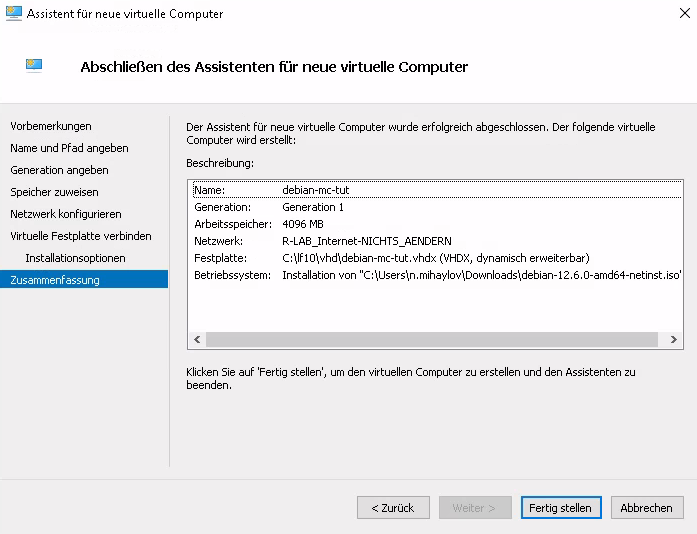
\includegraphics[width=1\textwidth]{vm-config}
\end{figure}
\FloatBarrier

\section{Acquiring the newest Debian 12 image}

The newest version of the Debian 12 image can be acquired from the official website \href{https://www.debian.org/download}{(click here for a link to the download page)}. You should note that we're using the netinst for this tutorial which requires an internet connection to download any additional packages, but you can also use a regular complete image for offline installation.

\section{Installation process}

The GUI-based installation should be relatively straight-forward - you can use the defaults and modify the hostname to your liking (here we're just going to use "debian-mc"). Debian's defaults will take of disk partitioning on our new VHDX. Make sure to select your appropriate time zone, locale and mirror region!

Some things to note for the installation process is to *not* install a desktop environment; we are only going to require an SSH connection to interface with our server as we want to avoid the overhead of any graphical environment, therefore you should only select "SSH server" and "standard system utilities" (refer to Figure 2. for a visual example).

\begin{figure}[h]
	\caption{Our Debian 12 software selection}
	\centering
	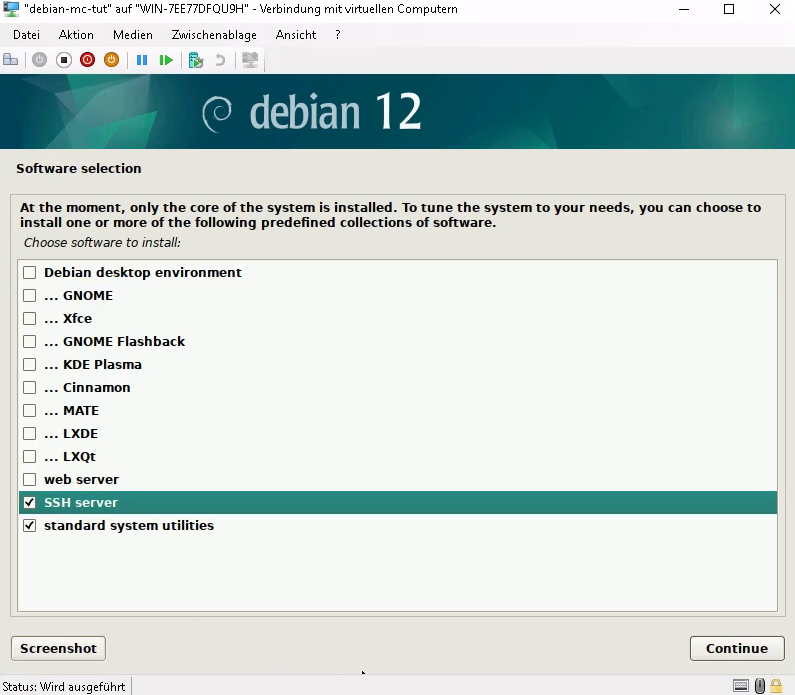
\includegraphics[width=1\textwidth]{debian-software-selection}
\end{figure}
\FloatBarrier

The reason why we're looking into having SSH out of the box is because it will make copying and pasting text much easier, and you will most likely need to do that later during the tutorial. Having a user with sudo privileges will be a prerequisite for SSH access, and now that you've made a user account during the installation all that's left in this regard is to add them to the sudo group post-install.

Once that is done, make sure to install the GRUB boot loader to your primary drive (/dev/sda), otherwise you won't be able to boot into your installation afterwards.

Now you should have a functioning Debian 12 installation with a TTY login prompt.

\begin{figure}[h!]
	\caption{The Debian 12 TTY prompt}
	\centering
	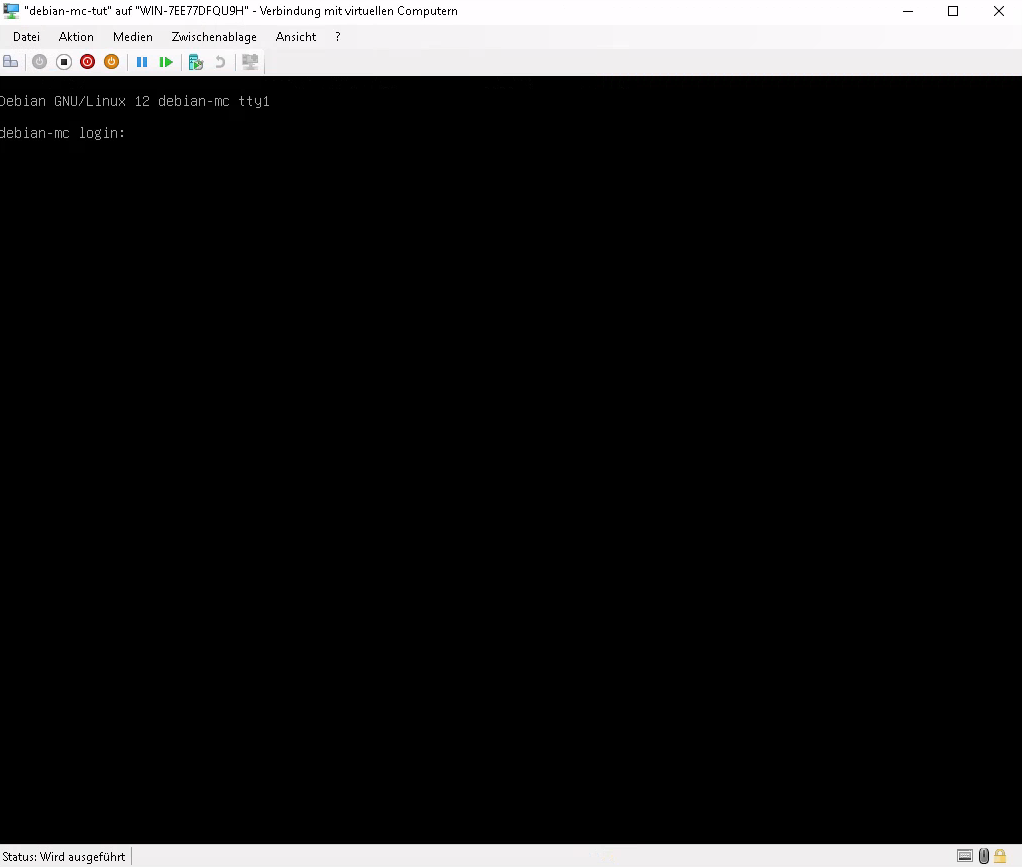
\includegraphics[width=1\textwidth]{tty}
\end{figure}
\FloatBarrier

\section{Initial post-installation configuration}

Before we begin with anything Minecraft-related, there are a couple of post-installation things to configure, with our first and most important one being giving our newly-created user sudo permissions. To do this, we log in as root:

\begin{verbatim}
	debian-mc login: root
	Password: {your-root-password-here}
\end{verbatim}

Now you should be logged in as root and facing the prompt.

First order of business is to install the sudo package if it is not already installed. To do this, we are going to type:

\begin{verbatim}
	apt install sudo
\end{verbatim}

The apt command is used to manage packages on the Debian system. With the "install" flag we can specify a package name to install, in this case the sudo package. If sudo wasn't available on your system already, your package manager will ask you if you want to install the package. Confirm it with enter. You can type sudo afterwards to confirm that the package has been installed with the output being the help for the command.

Now that that's done, we can continue with our preliminary configuration. We can list all users on the system with the following command:

\begin{verbatim}
	cat /etc/passwd
\end{verbatim}

Your newly-created user from the graphical installer will most likely be at the very bottom. Here you can see the local user entries per-line and their associated User ID (UID), Group ID (GID), home directory, default shell and more.

\begin{figure}[h!]
	\caption{Output of the /etc/passwd file}
	\centering
	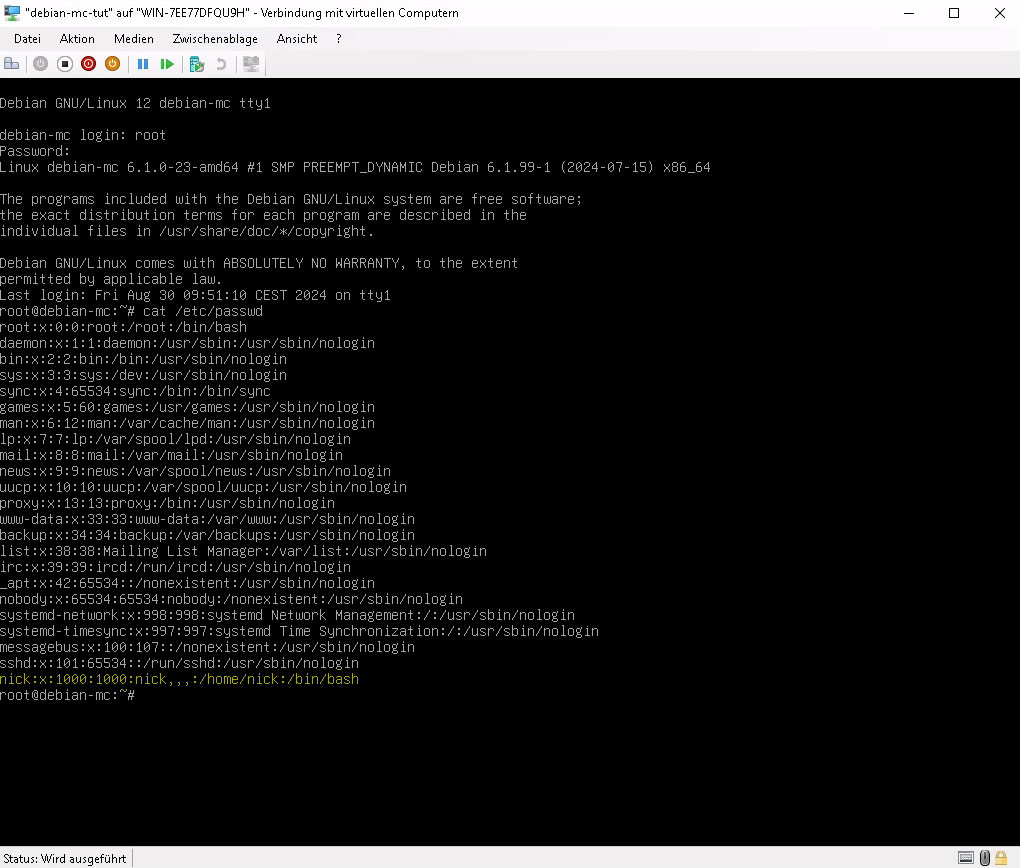
\includegraphics[width=1\textwidth]{passwd}
\end{figure}
\FloatBarrier

Now we are going to add our user to the sudo group. The sudo group is a special group which has administrative privileges using the sudo command. To do this, we are going to type the following:

\begin{verbatim}
	usermod -aG sudo {your-username-here}
\end{verbatim}

The usermod command allows us to modify the user entries we saw earlier in the /etc/passwd file. The -a option is for "append", i.e add a user to a group. The -G option is for specifying a group by its name (in this case sudo). In a lot of GNU/Linux tools you are able to combine options together like "-aG" instead of "-a -G". If you typed the command and received no output, that means it should be all good.

You can now switch back your user with the su (switch user) command to test your newly-given sudo privileges:

\begin{verbatim}
	su {your-username-here}
\end{verbatim}

Now try updating your system using sudo:

\begin{verbatim}
	sudo apt update && sudo apt upgrade
\end{verbatim}

If everything went well, you should be able to synchronize your system with the apt repository and install any available updates on your computer!

\begin{figure}[h!]
	\caption{Testing the newly-given sudo privileges by updating our system}
	\centering
	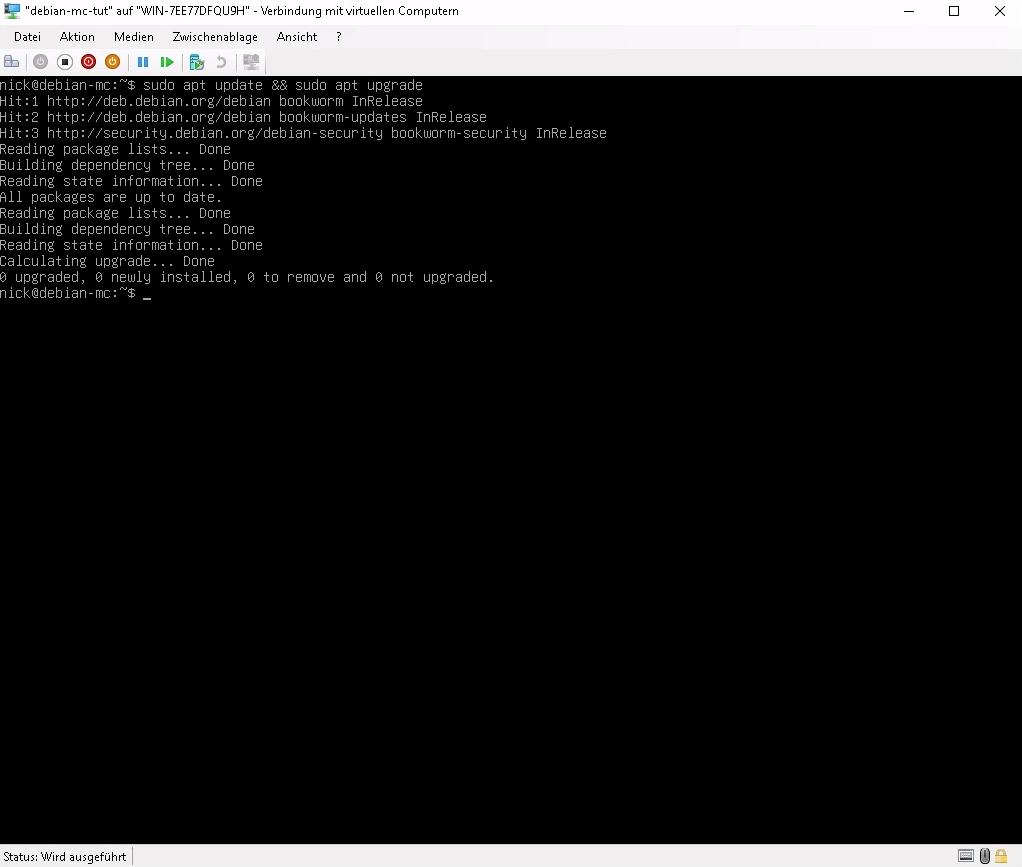
\includegraphics[width=1\textwidth]{update}
\end{figure}
\FloatBarrier

\section{Establishing an SSH connection}

If you followed the installation section of this tutorial, you most likely already have OpenSSH installed which is required for this section. To check it, you can issue the following command:

\begin{verbatim}
	ssh
\end{verbatim}

You will now get the command help output if the OpenSSH package is installed on your system. If not, install it with the following command:

\begin{verbatim}
	sudo apt install openssh-server
\end{verbatim}

Once that is done, we can hop back to our host system and open a command prompt (for example PowerShell). To establish a connection we must follow a specific syntax:

\begin{verbatim}
	ssh {username}@{ipv4-address}
\end{verbatim}

We connect as a user on our SSH server at the given IPv4 address of the server. If you don't know your IPv4, you can issue the following command to get the IPv4 of your ethernet adapter/NIC:

\begin{verbatim}
	ip addr | grep "eth0"
\end{verbatim}

The "ip addr" command outputs information on the network interfaces of the system. Because we're working with a VM, it is highly likely we're using a virtual ethernet adapter, hence the default "eth0" we're trying to get the information from. If you are to normally run "ip addr", it will output all interfaces which shouldn't be a problem on our fresh install, but when dealing with commands that output lots of information of which we only require a small amount of, we can simultaneously utilize the "grep" command. This utility scans the output of your previous command (in our case ip addr) and only outputs the line which is given as an argument to grep (this being "eth0").

The pipe between these two commands is the most important part; this should be your introduction to the concept of input/output redirection in Linux, with the pipe taking the output of our command to the left of it and providing it as an input to the command on the right. Vaguely said, the flow of this entire command is now \texttt{"ip addr" -> | -> "grep 'eth0'"}.

Your resulting output should be similar to this:

\begin{figure}[h!]
	\caption{The output of the \texttt{ip addr | grep "eth0"} command}
	\centering
	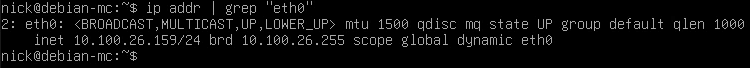
\includegraphics[width=1\textwidth]{ip-addr}
\end{figure}
\FloatBarrier

With our IP address in hand, we can now use our terminal emulator of choice and use the syntax from earlier to connect to our machine from our host:

\begin{figure}[h!]
	\caption{Establishing an SSH connection to the VM}
	\centering
	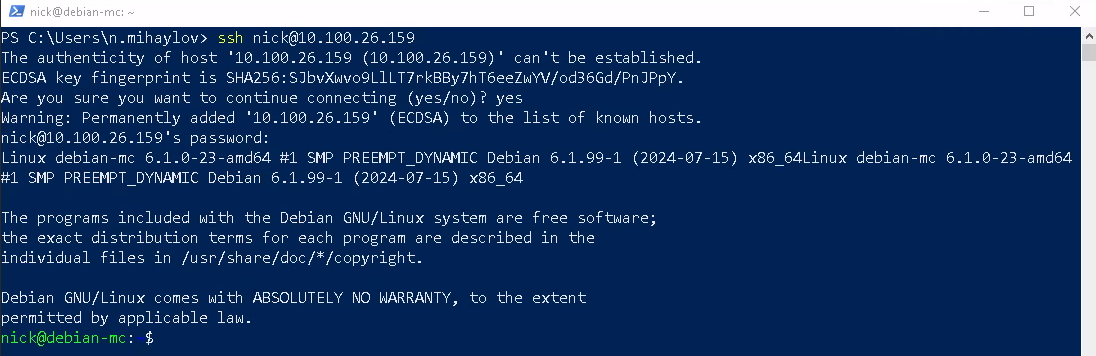
\includegraphics[width=1\textwidth]{ssh}
\end{figure}
\FloatBarrier

Success! You should now have an SSH connection to your Debian 12 virtual machine. Of course, it is important to note that the machines should be on the same network, but you can take this as far as using a terminal emulator on your GFN-issued laptop instead of RemoteLabs to connect to the VM via SSH. With this in hand you are now able to copy and paste lengthy commands easily into your VM without requiring to type them out manually.

\section{Preparing the Minecraft Forge server installation}

In order to host our instance of Forge for the Minecraft server we require an installation of the Java Development Kit on our system.

Here a problem arises: the most recent version of Forge requires version 21 of the JDK but this version of OpenJDK is still in the testing repository as of the time of writing this document, and the Oracle JDK is licensed under their own license and isn't available in the repositories either. This is where I must make it clear that this is not to be used in a production environment just because of how messy the current Java situation on Debian is.

With all that being said, this document will continue with the Oracle JDK 21 .deb file which can be found \href{https://www.oracle.com/java/technologies/downloads/}{(here)}. Copy the link to the .deb file from this page and keep it in your clipboard.

Back to the established SSH connection to our Debian 12, we need to create a folder to store our downloaded file. For this we're going to first navigate to our user's home folder by just typing "cd" (you can verify which directory you're currently in with the "pwd" command) and then use the "mkdir" command (make directory) within our home directory to create a new one like so:

\begin{verbatim}
	mkdir Downloads
\end{verbatim}

Now if we do an "ls" (list) we should see that the new directory with the name "Downloads" has been created.

\begin{figure}[h!]
	\caption{Creating a directory in the user's home}
	\centering
	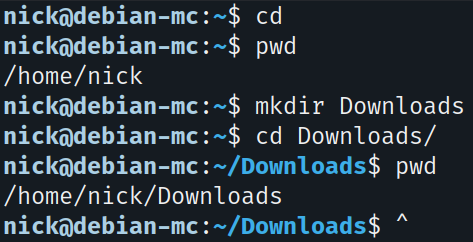
\includegraphics[width=1\textwidth]{downloads}
\end{figure}
\FloatBarrier

At this point we can download the JDK .deb file we currently have in our clipboard using the "wget" tool. The command should be pretty simple now that we have a functional clipboard at hand thanks to SSH:

\begin{verbatim}
	wget https://download.oracle.com/java/22/latest/jdk-22_linux-x64_bin.deb
\end{verbatim}

The link above is for the Oracle JDK 22. Depending on when you read this document, the OpenJDK 21 package might already be in the Debian stable repository. As for the rest of the tutorial, we will proceed with the downloaded .deb file from Oracle.

If you perform an "ls" in your Downloads directory you should see the file you just downloaded with "wget":

\begin{figure}[h!]
	\caption{The downloaded JDK .deb file}
	\centering
	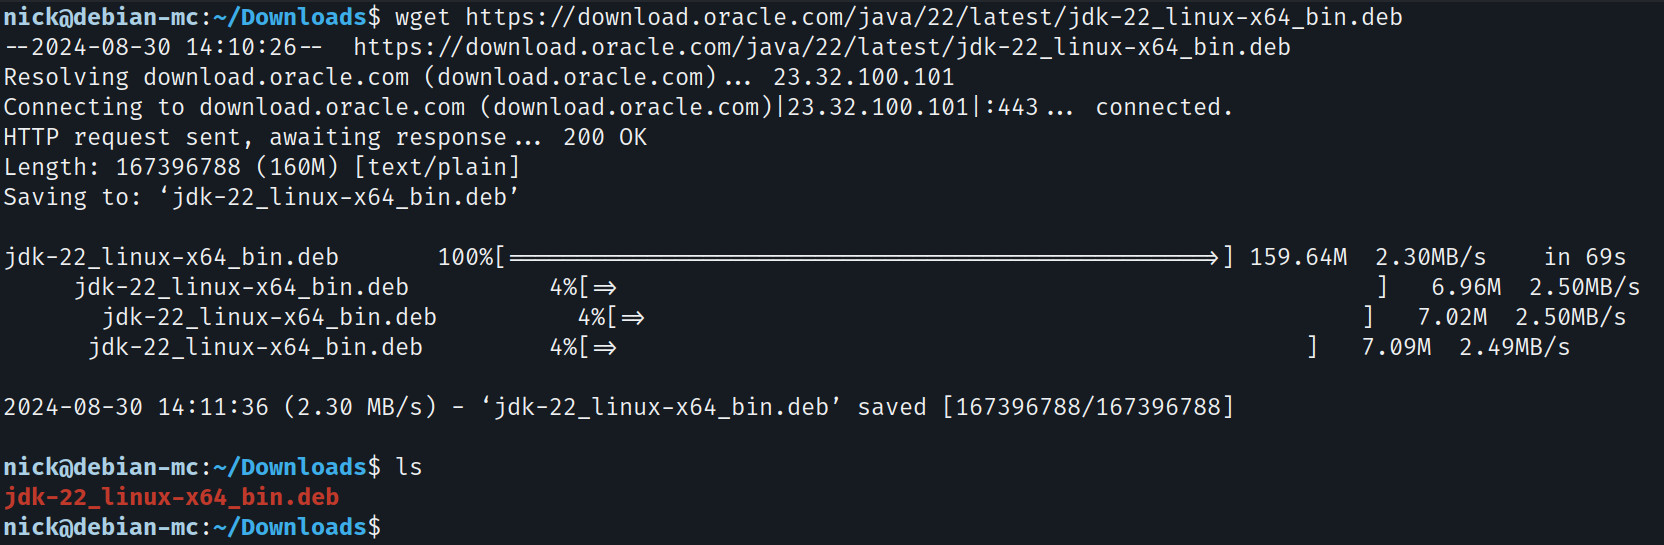
\includegraphics[width=1\textwidth]{wget}
\end{figure}
\FloatBarrier

Files with the .deb extension are not unlike a Windows .exe installer file - they contain the required binaries and data for an application as well as all necessary meta information for the system. As a matter of fact, you can open this file with an archive viewer and see that it consists of two tarball archives, each for the application itself and its metadata.

To install a .deb file as a system package, we will need the "dpkg" command. "apt" actually uses "dpkg" under the hood to perform the installation of packages, but right now we're skipping "apt" and going directly to "dpkg" to install a file. We're going to use the following command:

\begin{verbatim}
	sudo dpkg -i jdk-22_linux-x64_bin.deb
\end{verbatim}

Remember that you can use tab-complete! Start with the first few letters of the file name and use the Tab key to automatically fill in the rest. You will be prompted for your sudo password and installation should begin.

When the installation completes there will be all sorts of output on your terminal. If it looks similar to the following figure, you should be good to go.

\begin{figure}[h!]
	\caption{Output of the JDK .deb installation}
	\centering
	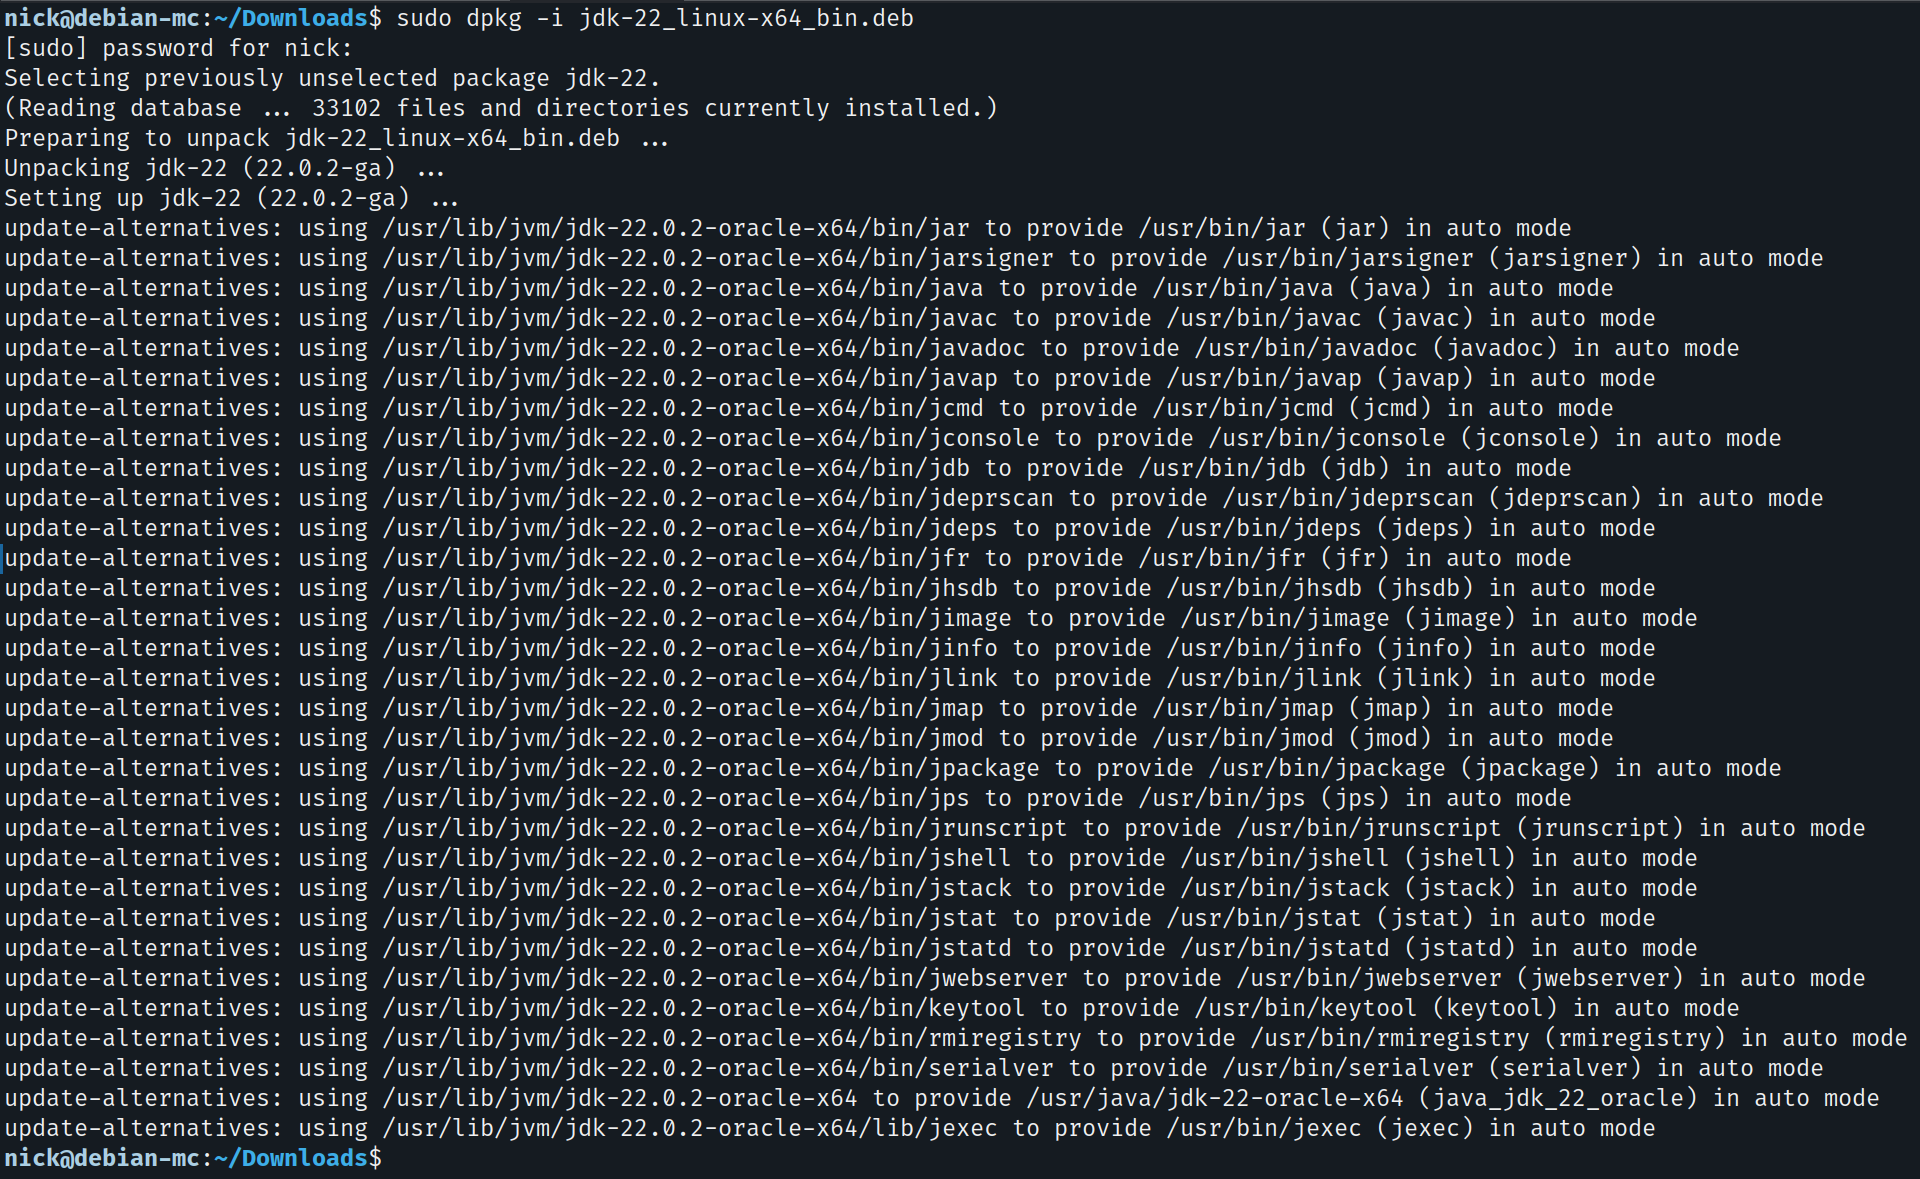
\includegraphics[width=1\textwidth]{jdk-output}
\end{figure}
\FloatBarrier

You can verify the installation by running \texttt{java --version} which will hopefully display the version of the package you just installed (in this case 22.0.2). You have now successfully installed the required Java JDK for running Forge!

\section{Installing Minecraft Forge}

We should first create a dedicated directory for our installation of Minecraft and cd into it:

\begin{verbatim}
	sudo mkdir /opt/minecraft
	cd /opt/minecraft
\end{verbatim}

Now using "wget" we can download the newest recommended version of Forge as of the time of writing this document which you can get from \href{https://maven.minecraftforge.net/net/minecraftforge/forge/1.20.6-50.1.0/forge-1.20.6-50.1.0-installer.jar}{(here)}. Running "wget" with this link as the argument will download the file in our \texttt{/opt/minecraft} directory:

\begin{verbatim}
	sudo wget https://maven.minecraftforge.net/net/minecraftforge/forge/1.20.6-50.1.0/forge-1.20.6-50.1.0-installer.jar
\end{verbatim}

Verify that the file has been downloaded in the current directory with an "ls". We can now proceed with installing the server version of Minecraft Forge with the .jar file using Java:

\begin{verbatim}
	sudo java -jar forge-1.20.6-50.1.0-installer.jar --installServer
\end{verbatim}

This process might take a little while. You will know it completed successfully by the  "The server installed successfully" message at the end.

The next step is to make an "eula.txt" file which is required by the Minecraft server. We can either "touch" the file to create it with no contents or create it using a text editor like "nano" as we will need to write contents into the file anyway.

"Touching" a file creates an empty file of the same name you provided to the touch command like so:

\begin{verbatim}
	sudo touch eula.txt
\end{verbatim}

Now when you "ls" the directory you should see the file. If you "cat" it to output its contents, you will see nothing as it is an empty file. To edit it we will use the "nano" text editor:

\begin{verbatim}
	sudo nano eula.txt
\end{verbatim}

You will now find yourself in the interface of the nano text editor:

\begin{figure}[h!]
	\caption{The nano text editor}
	\centering
	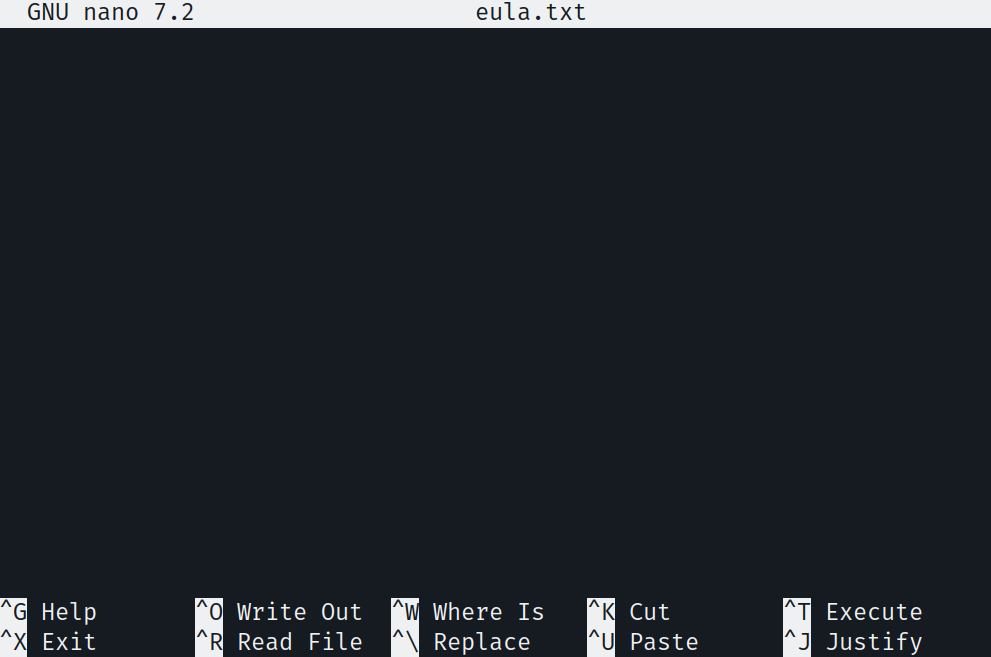
\includegraphics[width=1\textwidth]{nano}
\end{figure}
\FloatBarrier

nano is a relatively straight-forward text editor - you can start typing away to write text in the editor buffer and save it by pressing Ctrl+O to "write it out" and confirm with Enter. Here we only have to add the following line:

\begin{verbatim}
	eula=true
\end{verbatim}

Write the buffer out to the file by pressing Ctrl+O and hitting Enter to save under the default file name. If you face an error while saving you have most likely forgotten to start nano as a superuser with the sudo command.

If you're still in the mood for output redirection, we can skip using "nano" and make our Bash shell write this line to our file by using this command:

\begin{verbatim}
	echo "eula=true" | sudo tee -a eula.txt
\end{verbatim}

The "echo" command prints whatever comes after it to the shell, but the pipe takes this output and passes it to "tee" with sudo privileges to append it with the -a flag to the eula.txt file. "tee" command is a utility that reads an output of a command, display it on the screen and also write it into an output file (in this case the "eula.txt"). While it is more convenient to add this line to our file using a text editor like nano, the concept of redirection is important when it comes to creating scripts which may be useful for you eventually on your Linux journey.

We can verify the contents of the file with "cat" which should output what we just wrote in the file.

Now let's "touch" an empty "server.properties" file into existence:

\begin{verbatim}
	touch server.properties
\end{verbatim}

Let's also modify an existing file in this directory with the name \texttt{user\_jvm\_args.txt}. This should contain the instructions for how the Java Virtual Machine is to be started.

\begin{verbatim}
	sudo nano user_jvm_args.txt
\end{verbatim}

All lines starting with a \# are going to be ignored as they're interpreted as comments; whatever follows afterwards that doesn't have a \# will be read as a configuration file entry. All we need to add is the following:

\begin{verbatim}
	-Xms4G
	-Xmx4G
\end{verbatim}

This allocates a minimum and maximum of 4GB of RAM to the JVM. Note that the first X's are capitalized.

All that's left is to edit the "run.sh" shell script file to modify the very last line by prepending \texttt{cd /opt/minecraft \&\&} at the beginning of the line and adding a \texttt{nogui}.

Your file should now look like this:

\begin{figure}[h!]
	\caption{The contents of the edited run.sh file}
	\centering
	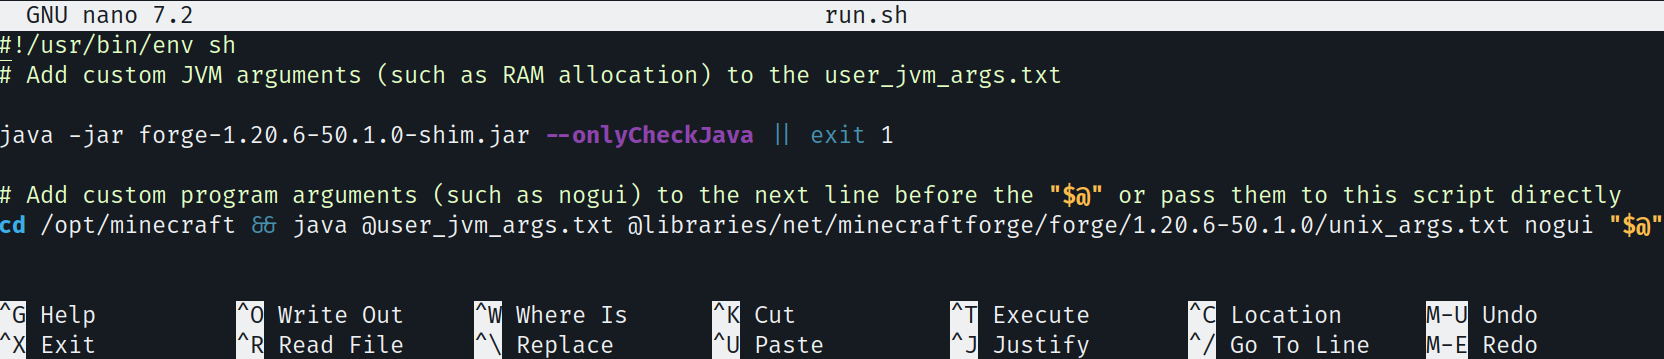
\includegraphics[width=1\textwidth]{run-sh}
\end{figure}
\FloatBarrier

With everything hopefully being finalized, we can at long last run the shell script to start our Minecraft server:

\begin{verbatim}
	sudo sh run.sh
\end{verbatim}

This process will take a while especially during the world generation stage. You will know it's done by "Done" message and the > of the Minecraft console prompt once everything is set up. You can now try connecting to your newly-created Minecraft server while keeping in mind you might need a specific version of the client (in this case I used the client version 1.26.0 which is managed by Prism Launcher).

\begin{figure}[h!]
	\caption{Joining the server using the IPv4 address}
	\centering
	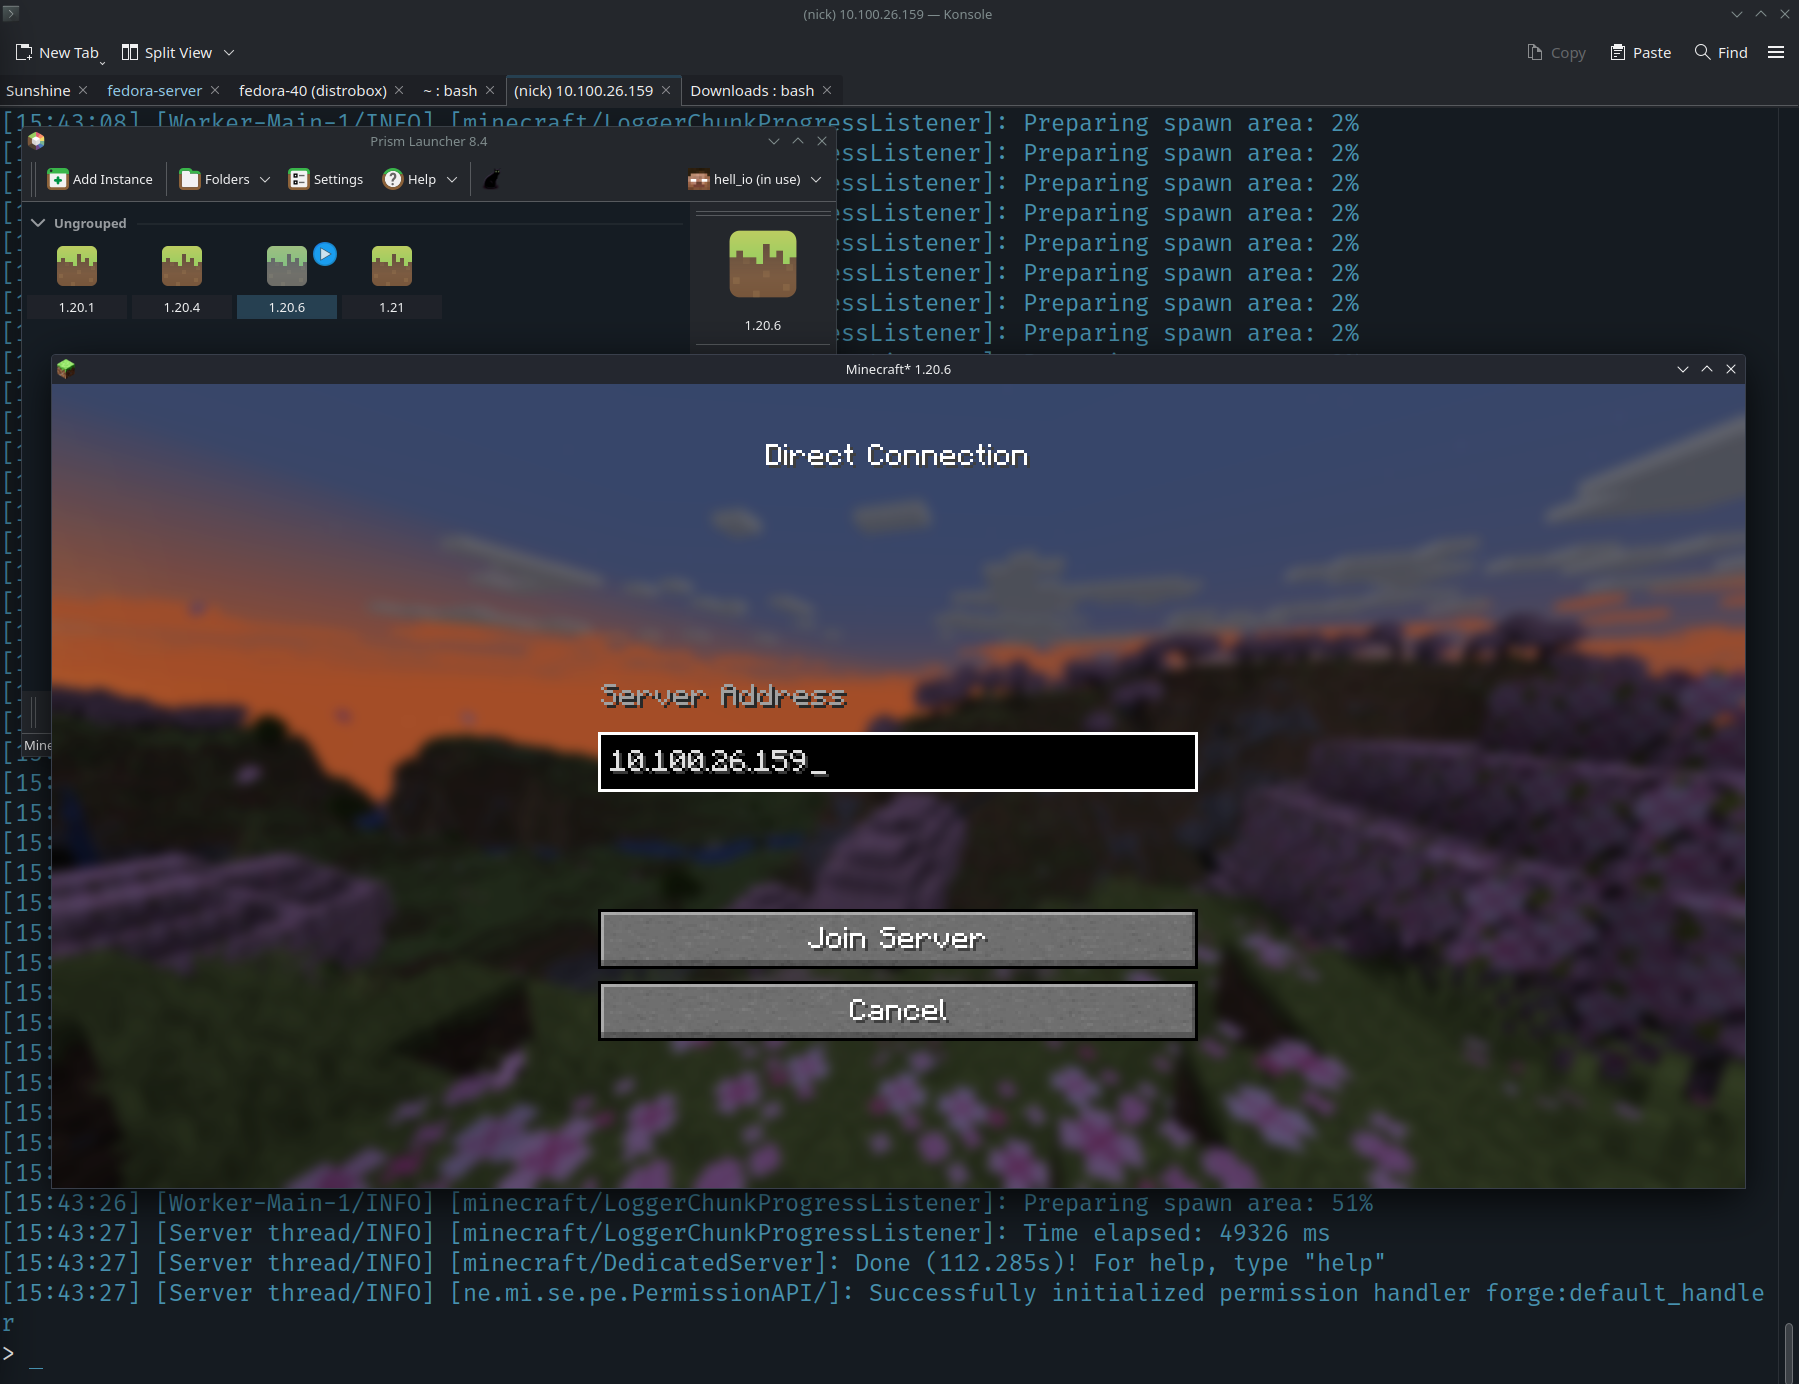
\includegraphics[width=0.8\textwidth]{mc-connect}
\end{figure}
\FloatBarrier

\begin{figure}[h!]
	\caption{In-game screenshot of the server and the generated seed}
	\centering
	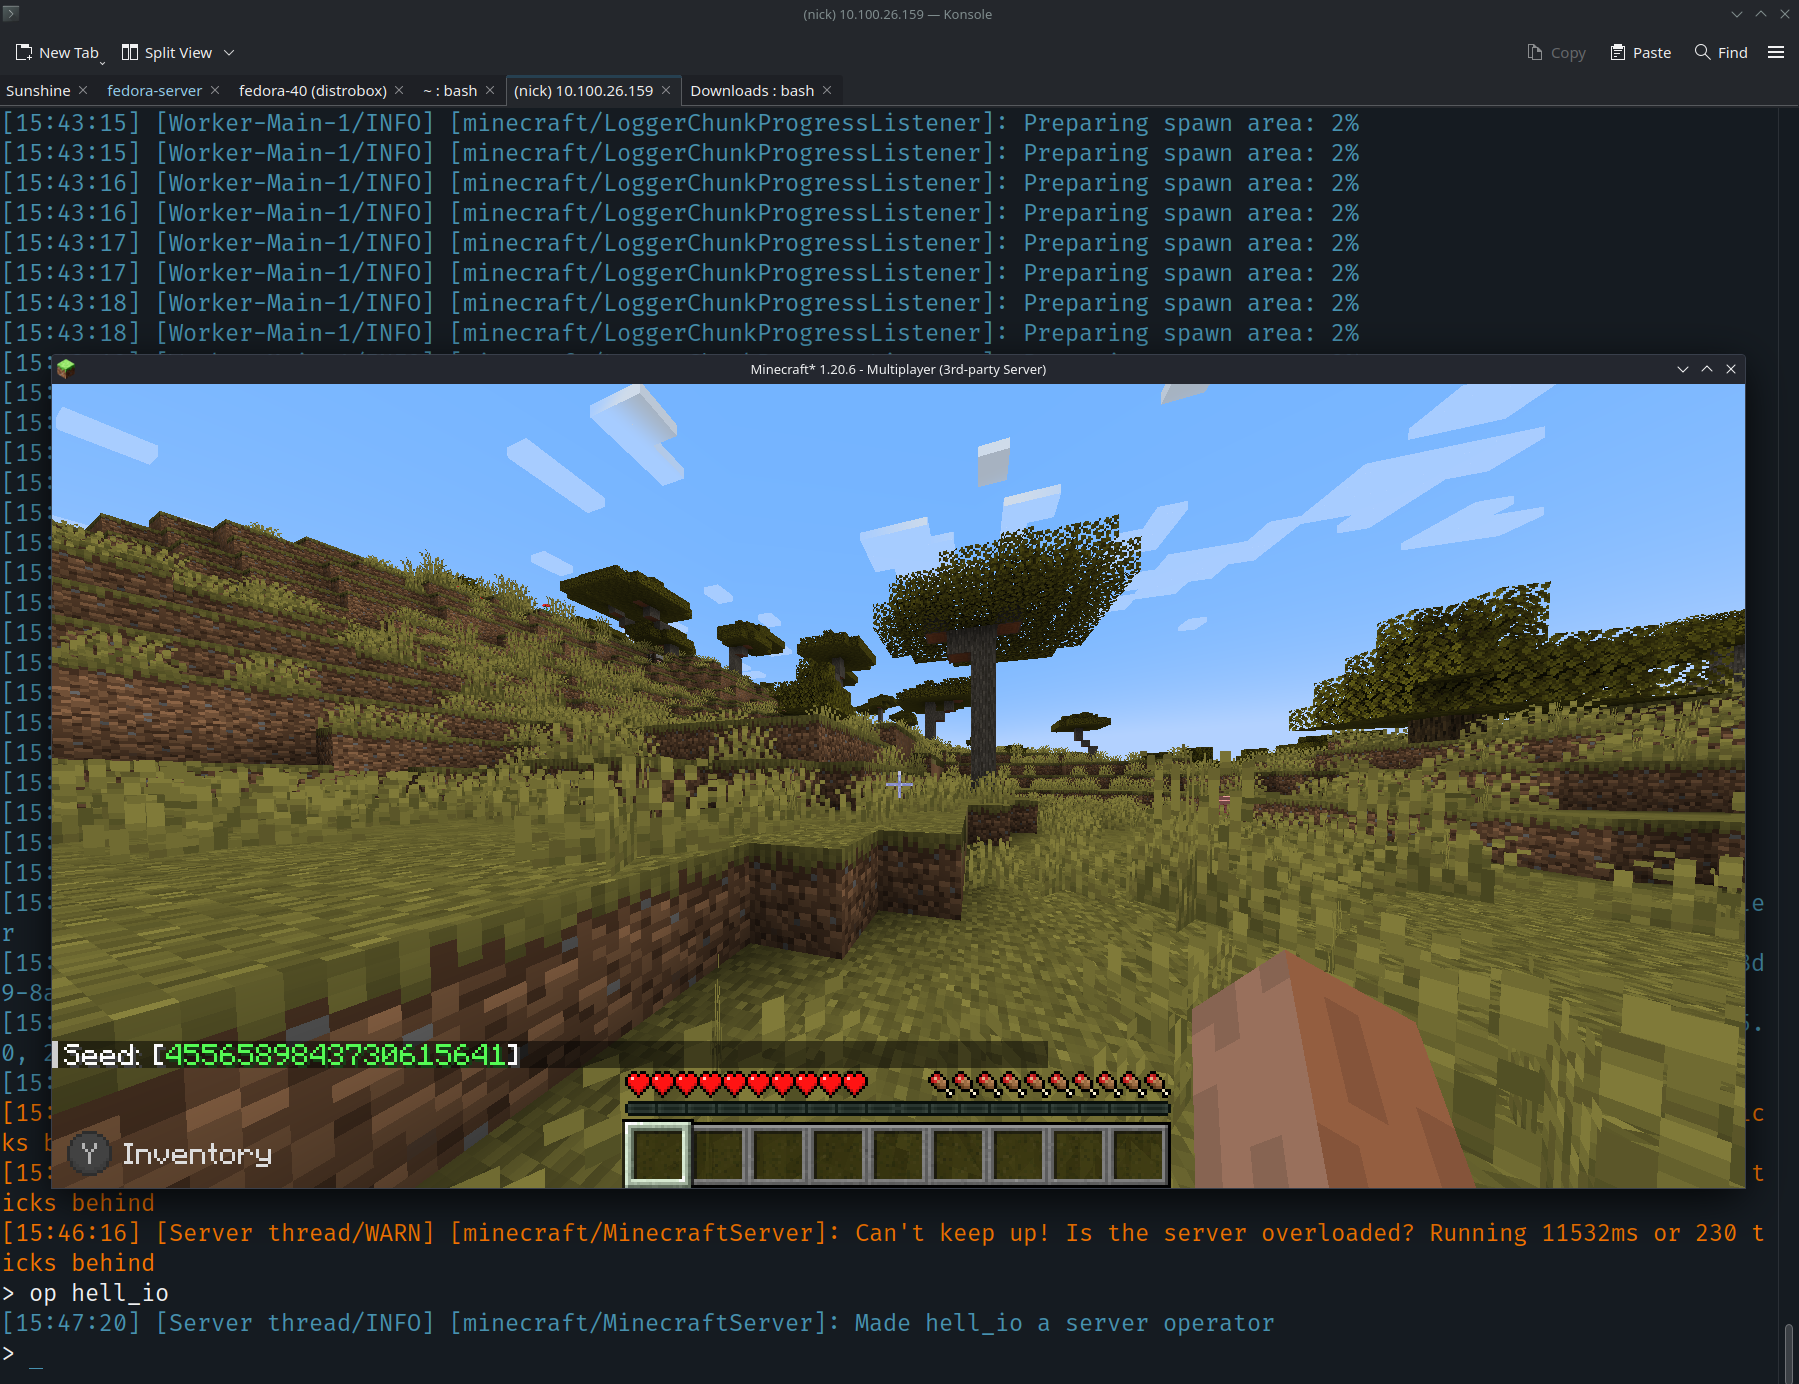
\includegraphics[width=0.8\textwidth]{mc-server}
\end{figure}
\FloatBarrier

Congratulations! You should now have a functioning Minecraft Forge server on your Debian 12 virtual machine!

\end{document}
